

\documentclass[
11pt, 
french, % ngerman for German
singlespacing, 
nohyperref, 
headsepline,
]{MastersDoctoralThesis} 


%\usepackage{accanthis}
\usepackage[utf8]{inputenc} % Required for inputting international characters
\usepackage[T1]{fontenc}
%\usepackage[T1,T2A]{fontenc} 
%\usepackage[utf-8]{inputenc}% Output font encoding for international characters
\usepackage{palatino} % Use the Palatino font by default
%\usepackage{fontspec}
%\setsansfont{Calibri}
% Set serifed font to Cambria
%\setmainfont{Cambria}
\usepackage{lmodern}
%\usepackage{wasysym}
\usepackage{soul}
\usepackage{amsthm}
\usepackage[fleqn]{amsmath}
\usepackage{mathtools}
\usepackage{amsfonts}
\usepackage{amssymb}
\usepackage{ragged2e}
\usepackage{graphicx}
\usepackage[justification=justified, margin=10pt]{caption}
\usepackage{titlesec}
\usepackage{enumitem}
\usepackage{multirow}
\usepackage{tabularx}
\usepackage{url}
\usepackage{subfig}
\usepackage{listings}
\usepackage{changebar}

\newcommand{\code}[1]{{\small\tt #1}}
%\usepackage{tikz}

\lstset{
	basicstyle=\ttfamily\tiny
}

%-----------------------------------------------------------------------------
% ****************This so the table will work **********************************
\DeclareUnicodeCharacter{00A0}{~}
% %****************************************************************************
%-------------------------------------------------------------------------------


\frenchbsetup{StandardLists=true}
\usepackage[autostyle=true]{csquotes} % Required to generate language-dependent quotes in the bibliography
\usepackage{hyperref}
\usepackage[usenames,dvipsnames,svgnames,table]{xcolor}

%%%%% Style of hyperref  %%%%%%
\usepackage{hyperref}
\hypersetup{
     colorlinks=true,
     linkcolor=blue,
     urlcolor=blue,
     citecolor=gray
}
%%%%%%%%%%%%%%%%%%%%%%%%%%%%%%%%%

%%%% Style of caption %%%%%%%%%%%
%\usepackage{subcaption}
\captionsetup{compatibility=false}
%eps to pdf
\usepackage{epstopdf}
%%%%%%%%%%%%%%%%%%%%%%%%%%%%%%%%%

%%%%%% Style of bibliography %%%%%%%%%%%%%%%%%%%%%%%%%%%%%%%%%
\usepackage[backend=bibtex,style=alphabetic, sorting=none]{biblatex} % Use the bibtex backend with the authoryear citation style (which resembles APA)
\bibliography{biblio}
%%%%%%%%%%%%%%%%%%%%%%%%%%%%%%%%%%%%%%%%%%%%%%%%%%%%%%%%%%%%%%%



%----------------------------------------------------------------------------------------
%	MARGIN SETTINGS
%----------------------------------------------------------------------------------------

\geometry{
	paper=a4paper, % Change to letterpaper for US letter
	inner=2.5cm, % Inner margin
	outer=2.5cm, % Outer margin
	bindingoffset=0cm, % Binding offset
	top=1.5cm, % Top margin
	bottom=1.5cm, % Bottom margin
	%showframe,% show how the type block is set on the page
}

%%%%%%% Font Settings %%%%%%%%%%%%%%%%%%%%%%%%%%%%%%%
%\begin{myfont}
\definecolor{gray75}{gray}{0.75}
\definecolor{myblue}{RGB}{34,58,109}
\definecolor{2ndblue}{RGB}{44, 109, 189}
\newcommand{\hsp}{\hspace{20pt}}
%\titleformat{\chapter}[hang]{\Huge\bfseries}{\thechapter\hsp\textcolor{gray75}{|}\hsp}{0pt}{\Huge\bfseries}


%\titleformat{\chapter}[shape]{format}{label}{sep}{before-code}{after-code}



\titleformat{\chapter}[block]
{\Huge}{\bfseries\textcolor{myblue}{\thechapter}\textcolor{myblue}{\textbf{|}}\hsp}{0pt}{\centering\Huge\scshape}
[\vspace{-1ex}%
\rule{\textwidth}{2.5pt}] 
		
	%{	\rule{\textwidth}{2pt}
%		\vspace{0ex}
%		\centering} % before-code
%	[\vspace{-0.5ex}%
%	\rule{\textwidth}{2.5pt}] % after-code


%\titleformat
%{\chapter} % command
%[block] % shape
%{\Huge\bfseries} % format
%{\textcolor{myblue} {\thechapter \hsp\textcolor{myblue}{\textbf{|}}\hsp}} {0.5ex} {	\rule{\textwidth}{2pt}
%	\vspace{0ex}
%	\centering} % before-code
%[\vspace{-0.5ex}%
%\rule{\textwidth}{2.5pt}] % after-code



\titleformat{\section}[block]
{\normalfont\Large\bfseries \color{black}}
{\thesection}
{1em}{}




\titleformat{\subsection}[block]
{\normalfont\large\bfseries\color{black}}
{\thesubsection}
{1em}{}
%\end{myfont}
%%%%%%%%%%%%%%%%%%%%%%%%%%%%%%%%%%%%%%%%%%%%%%%%%%%%%%



%%%% Definitions, lemmas, corollaries and theorems
\newcounter{dummy} \numberwithin{dummy}{chapter}

\usepackage[framemethod=tikz]{mdframed}
\newmdtheoremenv[
hidealllines=true,
leftline=true,
innertopmargin=0pt,
innerbottommargin=0pt,
linewidth=4pt,
linecolor=gray!40,
innerrightmargin=0pt,
]{dfn}[dummy]{Definition}
\let\olddefinition\dfn
\renewcommand{\dfn}{\olddefinition\normalfont}


\newmdtheoremenv[
hidealllines=true,
leftline=true,
innertopmargin=0pt,
innerbottommargin=0pt,
linewidth=4pt,
linecolor=gray!40,
innerrightmargin=0pt,
]{lem}[dummy]{Lemma}
%\renewcommand{lem}[dummy]{lemm}
\let\oldlemma\lem
\renewcommand{\lem}{\oldlemma\normalfont}

\newmdtheoremenv[
hidealllines=true,
leftline=true,
innertopmargin=0pt,
innerbottommargin=0pt,
linewidth=4pt,
linecolor=gray!40,
innerrightmargin=0pt,
]{thm}{Theorem}
\let\oldtheorem\thm
\renewcommand{\thm}{\oldtheorem\normalfont}
\numberwithin{thm}{chapter}

\theoremstyle{definition}
\newtheorem{exmp}{Example}[chapter]

\newtheorem*{remark}{Remark}


% Numbering in roman style
\renewcommand\thechapter{\arabic{chapter}}
\renewcommand\thesection{\thechapter.\arabic{section}}
\renewcommand\thesubsection{\thesection.\arabic{subsection}}
\renewcommand\theequation{{\color{blue}\thechapter.\arabic{equation}}}


\renewcommand{\arraystretch}{1.5}

\newcommand{\KB}[1]{\hl{#1}}

%\usepackage[Lenny]{fncychap}



\hypersetup{
     colorlinks=true,
     linkcolor=blue,
     urlcolor=blue,
     citecolor=gray
}


%----------------------------------------------------------------------------------------
%	THESIS INFORMATION
%----------------------------------------------------------------------------------------

\thesistitle{Dossier de candidature au prix de thèse GDR GPL 2020} % Your thesis title

\supervisor{} 
\examiner{} 
\degree{} 
\author{} 
\addresses{} 
\subject{} % 
\keywords{} 
\university{\href{http://www.ec-nantes.fr/}{Université de Nantes}} 
\department{\href{http://department.university.com}{Department or School Name}} 
\group{\href{http://researchgroup.university.com}{Research Group Name}} 
\faculty{\href{http://faculty.university.com}{Faculty Name}} 
\hypersetup{pdftitle=\ttitle} 
\hypersetup{pdfauthor=\authorname}
\hypersetup{pdfkeywords=\keywordnames} 



\begin{document}
	
	%\pgfversion
\sloppy
\frontmatter % Use roman page numbering style (i, ii, iii, iv...) for the pre-content pages

\pagestyle{plain} % Default to the plain heading style until the thesis style is called for the body content




%----------------------------------------------------------------------------------------
%	THESIS CONTENT - CHAPTERS
%----------------------------------------------------------------------------------------

\mainmatter % Begin numeric (1,2,3...) page numbering

\pagestyle{thesis} % Return the page headers back to the "thesis" style



%\HRule \\[0.4cm] % Horizontal line
%{\huge \bfseries \chapter{Introduction}\par}\vspace{-0.9cm} % Thesis title
%\HRule % Horizontal line
\let\cleardoublepage\clearpage
\chapter{Curriculum Vit\ae{}}

\begin{center}
{\huge  \textbf{\textcolor{myblue} {Khaoula} \textcolor{myblue}{BOUKIR}}}
\vspace{0.4cm}

%\textcolor{myblue}{{\normalsize \textbf{{\Large P}\textcolor{2ndblue}{OST-DOCTORANTE EN} {\Large I}\textcolor{2ndblue}{NFORMATIQUE AU }{\Large CEA }\textcolor{2ndblue}{ DE }{\Large S}\textcolor{2ndblue}{ACLAY}}}}

\textcolor{2ndblue}{{\normalsize \textbf{{\Large P}\textcolor{2ndblue}{OST-DOCTORANTE AU }{\Large CEA }\textcolor{2ndblue}{ DE }{\Large S}\textcolor{2ndblue}{ACLAY}}}}


%Département Ingénierie Logiciels et Systèmes - \textit{DILS}
%
%Laboratoire pour la sûreté du logiciel - \textit{LSL}

 
 \vspace{0.3cm}
 
 \begin{minipage}{0.3\textwidth}
 	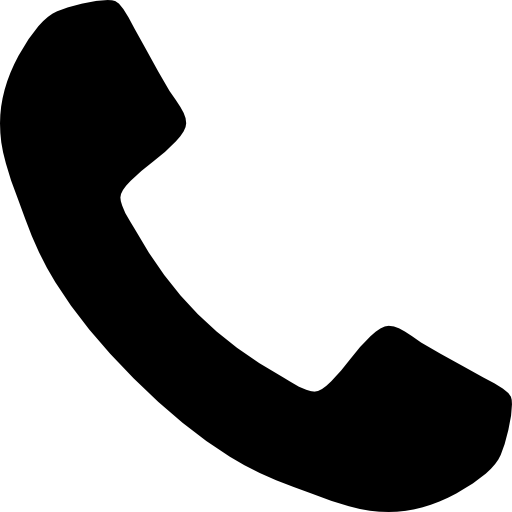
\includegraphics[width=0.1\textwidth]{Figures/tel.png} +33 (0)7 81 83 01 98
 \end{minipage}
 \begin{minipage}{0.4\textwidth}
 	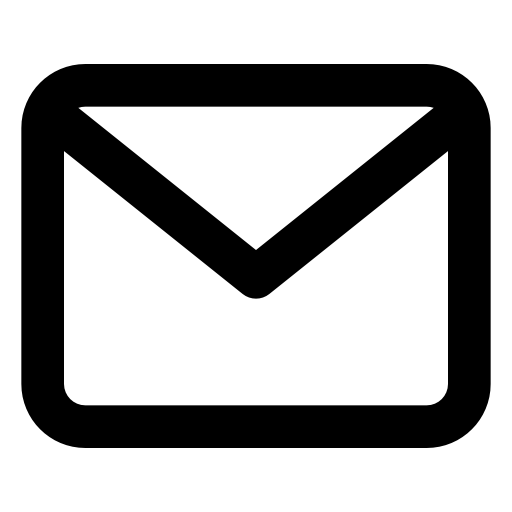
\includegraphics[width=0.1\textwidth]{Figures/mel.png} \url{boukir.khaoula@gmail.com}
 \end{minipage}


\vspace{0.3cm}



\includegraphics[width=0.04\textwidth]{Figures/web.png} \hspace{0.1cm} \url{https://khaoulaboukir.github.io/}

\end{center}


\begin{minipage}{0.2\textwidth}
	
\includegraphics[width=0.7\textwidth]{Figures/photo_id.jpg}
\end{minipage}\hspace{-1.5cm}
\begin{minipage}{0.7\textwidth}
	\begin{minipage}{0.5\textwidth}
		\begin{flushright}
			\textbf{	Nationalité :}
			
			\textbf{	Date de Naissance :}
				
			\textbf{	Lieu de Naissance :}
				
			\textbf{	Situation matrimoniale :}
				
		\textbf{		Adresse personnelle :}
		\end{flushright}
	
	\end{minipage}\hspace{0.4cm}
	\begin{minipage}{0.6\textwidth}
		
			Française
			 
			 27/06/1991 (29 ans)
			
			El Jadida (Maroc)
			
			Célibataire
			
			10 rue de chartres, 91400, Orsay
	\end{minipage}

\end{minipage}

%\textcolor{myblue}{\rule{\textwidth}{1.5pt}}
\vspace{0.5cm}

\section{Situation actuelle et antérieure}
\vspace{-0.6cm}
\hspace{0.7cm}\textcolor{myblue}{\rule{15cm}{1mm}}

\vspace{0.5cm}

Depuis Janvier 2021, je suis en poste de recherche post-doctorale au sein du CEA Paris-Saclay à temps plein dans le Laboratoire pour la Sûreté du Logiciel (\textit{LSL}) du Département Ingénierie Logiciels et Systèmes (\textit{DILS}). Je suis chargée de l'étude suivante : \og Analyse approfondie pour la sécurité des codes avec Frama-C \fg.

L'année précédente, j'ai travaillé en qualité d'Attachée Temporaire d'Enseignement et de Recherche (ATER) à temps plein aux deux départements Informatique et PeiP (Parcours des écoles d'ingénieurs Polytech) de Polytech'Nantes.


\section{Formation Académique}
\vspace{-0.6cm}
\hspace{0.7cm}\textcolor{myblue}{\rule{15cm}{1mm}}

\vspace{0.5cm}


\hspace{-0.7cm}\textbf{Octobre 2016 - Décembre 2020}

		\textbf{\textsc{Thèse de doctorat en Informatique Temps Réel}} à l'Université de Nantes, Nantes - France.
		\begin{itemize}[label=-]
			\itemsep0em 
			
			\item \textit{Sujet de thèse }: mise en œuvre de politiques d'ordonnancement temps réel prouvées.
			
			\item \textit{Directeur de thèse }: Jean-Luc B\'{E}CHENNEC, Chargé de recherche CNRS, \url{jean-luc.bechennec@ls2n.fr}.
			
			\item \textit{Co-encadrante }: Anne-Marie D\'{E}PLANCHE, Maître de conférence à l'Université de Nantes, \url{anne-marie.deplanche@ls2n.fr}.
			
			\item\textit{Laboratoire de rattachement} : Laboratoire des Sciences du Numérique de Nantes.
			
			\item\textit{École doctorale} : ED MathSTIC \footnotemark
			
		\end{itemize}

	\footnotetext{www.ed-mathstic.u-bretagneloire.fr}



\hspace{-0.7cm}\textbf{2015 - 2016}

		\textbf{\textsc{Master 2 recherche}} à l'\'{E}cole Centrale de Nantes, Nantes - France.
		\begin{itemize}[label=-]
			\itemsep-0em 
			\item \textit{Titre }: Automatique, Robotique et Informatique Appliquée, \textit{spécialité} : "Temps Réel, Conduite et Supervision", \textit{parcours} : "Systèmes Temps Réel".
			
			\item \textit{Classement }: \textbf{2ème}  du tronc commun, \textbf{Major} en spécialité. 
		\end{itemize}


\hspace{-0.7cm}\textbf{2012 - 2014}

		\textbf{\textsc{Formation d'Ingénieur d'état}} à l'\'{E}cole Nationale des Sciences Appliquées, Fès - Maroc.
		\begin{itemize}[label=-]
			\itemsep0em 
			\item \textit{Spécialité }: Génie des Réseaux et Télécommunications.
			
			\item \textit{Classement }: \textbf{Major de la promotion}.
		\end{itemize}


\hspace{-0.7cm}\textbf{2009 - 2012}

		\textbf{\textsc{Licence des Sciences et Techniques}} à la Faculté des Sciences et Techniques, Fès - Maroc.
		\begin{itemize}[label=-]
			\itemsep0em 
			\item \textit{Spécialité }: \'{E}.lectronique, Télécommunication et Informatique.
			
			\item \textit{Classement }: \textbf{Major de la promotion}.
		\end{itemize}


\section{Expériences}
\vspace{-0.6cm}
\hspace{0.7cm}\textcolor{myblue}{\rule{15cm}{1mm}}

\vspace{0.5cm}


\hspace{-0.7cm}\textbf{20/01/2021 - Aujourd'hui}

Poste de postdoctorante en informatique.
\begin{itemize}
	\item \textbf{Sujet :} analyse approfondie pour la sécurité des codes avec Frama-C.
	
	\item\textbf{ Superviseur : } Julien Signoles, Ingénieur de recherche au CEA, \url{Julien.Signoles@cea.fr}.  
\end{itemize}


\hspace{-0.7cm}\textbf{01/09/2019 - 31/08/2020}

		Poste d'Attachée Temporaire d'Enseignement et de Recherche en informatique.
		\begin{itemize}
			\item \textbf{Enseignement :} à l'école d'ingénieur Polytech'Nantes \url{<www.polytech.univ-nantes.fr>} - Départements : informatique et PeiP.
			
			\item\textbf{ Recherche : } Doctorante au Laboratoire des Sciences du Numérique de Nantes \url{<www.ls2n.fr>} - Équipe : Systèmes Temps Réel.
		\end{itemize}



\hspace{-0.7cm}\textbf{01/09/2017 - 31/08/2019}

		Contrat doctoral d'enseignement en électronique et informatique industrielle.
		\begin{itemize}
			\item \textbf{Enseignement :} à l'IUT de Nantes \url{<www.iutnantes.univ-nantes.fr>} - Département génie électronique et informatique industrielle.
		\end{itemize}



\hspace{-0.7cm}\textbf{01/09/2016 - 31/08/2017}

		Enseignante vacataire en informatique.
		\begin{itemize}
			\item \textbf{Enseignement :} à l'École Centrale de Nantes \url{<www.ec-nantes.fr>} - Département informatique.
		\end{itemize}



\hspace{-0.7cm}\textbf{01/10/2015 - 31/07/2016}

		Initiation à la recherche dans le cadre du Master 2 ARIA, au sein de l’équipe STR du LS2N, sous la direction de Mme Anne-Marie Déplanche.
		
		\begin{itemize}[label=-]
			\itemsep0em 
			\item \textbf{Séminaire bibliographique }: Etude de la politique U-EDF \cite{nelissen2012u} pour l’ordonnancement temps réel multiprocesseur.
			
			\item \textbf{Stage de recherche }: Mise en œuvre d’un ordonnanceur global dans l’OS temps
			réel Trampoline \cite{bechennec2006trampoline}.
		\end{itemize}


\hspace{-0.7cm}\textbf{19/12/2014 - 19/04/2015}

	Ingénieur Réseaux freelance au sein du groupe Hala à Fès.

\vspace{0.4cm}


\hspace{-0.7cm}\textbf{01/03/2014 - 30/06/2014}

		Stage de fin d’études, Huawei Technologies, Rabat - Maroc, \textit{sujet} : « Optimisation de la boucle du Nord de Maroc Telecom avec la nouvelle génération WDM et intégration d’une interface mobile pour sa supervision ».

\vspace{0.4cm}
\hspace{-0.7cm}\textbf{04/07/2013 - 04/09/2013}

		Stage d’application, Fedaso, Fès - Maroc, \textit{sujet} : « Développement d’une attaque	cybernétique de type déni de service sur un système d’information ».

\vspace{0.4cm}
\hspace{-0.7cm}\textbf{09/04/2012 - 05/06/2012}

		Stage de fin d’études, Office Chérifien des Phosphates, El Jadida - Maroc, \textit{Sujet} :
		« Elaboration d’un programme pour l’automatisation et la supervision du groupe de
		motopompes principales ».

\vspace{0.4cm}
\hspace{-0.7cm}\textbf{03/08/2010 - 02/09/2010}

		Stage d’initiation, Compagnie des Boissons Gazeuses du Nord, Fès - Maroc.

\vspace{0.4cm}
\hspace{-0.7cm}\textbf{15/06/2010 - 15/07/2010}

		Stage d’initiation, Office Nationale d’Électricité, Fès - Maroc.



\section{Compétences}
\vspace{-0.6cm}
\hspace{0.7cm}\textcolor{myblue}{\rule{15cm}{1mm}}

\vspace{0.5cm}

\begin{minipage}{0.08\textwidth}
	\hspace{0.1cm}
\end{minipage}
\begin{minipage}{0.9\textwidth}
	\begin{itemize}[label=\textbf{Enseignement}]
		\item	Programmation orientée objet - Algorithmique et programmation - Systèmes temps réel - Systèmes d'exploitation - Systèmes électroniques - Outils logiciels pour l'électronique - Logique classique - .
	\end{itemize}
	
	\begin{itemize}[label=\textbf{Recherche}]
		\item	Systèmes temps réel - Ordonnancement temps réel - Systèmes d'exploitation temps réel - Application des méthodes formelles pour la vérification des systèmes d'exploitation temps réel - Model-checking - Implémentation de politiques d'ordonnancement temps réel.
	\end{itemize}
	
	\begin{itemize}[label=\textbf{Langages}]
		\item	C/C++ - Python - Assembleur - HTML/CSS.
	\end{itemize}
	
	\begin{itemize}[label=\textbf{Logiciels}]
		\item CodeBlocks - Visual Studio - Atmel AVR Studio - Eclipse - DevC++ - Matlab (programmation), Uppaal - Roméo (model-checking), Simulink, ADS, Atoll, Comsis (simulateur de liaison électrique/télécom), Simso (simulateur d'ordonnanceur multiprocesseur)
	\end{itemize}
	
	\begin{itemize}[label=\textbf{Langues}]
		\item	Anglais, Français, Arabe (bilingue)
	\end{itemize}
	
	
	
\end{minipage}

\newpage
\section{Publications} \label{sec:publi}
\vspace{-0.6cm}
\hspace{0.7cm}\textcolor{myblue}{\rule{15cm}{1mm}}

%\vspace{0.7cm}

\begin{itemize}
	\item \textbf{{\Large Conférences internationales avec comité de lecture }}	
\end{itemize}

\begin{minipage}{0.08\textwidth}
	\hspace{0.1cm}
\end{minipage}
\begin{minipage}{0.9\textwidth}
	
	\begin{itemize}[label=\cite{boukir2020requirement}]
		\item	\textbf{Requirement specification and model-checking of a real-time scheduler implementation}
		
		Khaoula BOUKIR, Jean-Luc B\'{E}CHENNEC, Anne-Marie D\'{E}PLANCHE
		
		28th International Conference on Real-Time Networks and Systems (RTNS'20)
		
		
		
	\end{itemize}
	
	\begin{itemize}[label=	\cite{boukir2018formal} ]
		\item	\textbf{Formal approach for a verified implementation of Global EDF in Trampoline}
		
		Khaoula BOUKIR, Jean-Luc B\'{E}CHENNEC, Anne-Marie D\'{E}PLANCHE
		
		26th International Conference on Real-Time Networks and Systems (RTNS'18)
	\end{itemize}
	
	\begin{itemize}[label=	\cite{boukir2017reducing}]
		\item	\textbf{Reducing the gap between theory and practice: : towards a proven implementation of Global EDF in Trampoline}
		
		(\textit{Best paper award})
		
		Khaoula BOUKIR, Jean-Luc B\'{E}CHENNEC, Anne-Marie D\'{E}PLANCHE
		
		11th Junior Researcher Workshop on Real-Time Computing (JRWRTC'17) en conjonction avec RTNS'17.
	\end{itemize}
\end{minipage}

\begin{itemize}
	\item \textbf{{\Large Conférences nationales : }}	
	
	
\end{itemize}

\begin{minipage}{0.08\textwidth}
	\hspace{0.1cm}
\end{minipage}
\begin{minipage}{0.9\textwidth}
\begin{itemize}[label=	\cite{boukir2019}]
	\item	\textbf{Vérification d’une implémentation d’ordonnanceur temps réel par	model-checking}
	
	Khaoula BOUKIR, Jean-Luc B\'{E}CHENNEC, Anne-Marie D\'{E}PLANCHE
	
	13th GDR SOC2 National Symposium (GDR SOC2 2019).
\end{itemize}
\end{minipage}

\begin{itemize}
	\item \textbf{{\Large Comité de lecture }} 12th Junior Researcher Workshop on Real-Time Computing (JRWRTC'18) en conjonction avec RTNS'18.
\end{itemize}



\section{Activités para-académiques}
\vspace{-0.6cm}
\hspace{0.7cm}\textcolor{myblue}{\rule{15cm}{1mm}}

\vspace{0.3cm}

\begin{itemize}
	\item \textbf{2ème prix} au concours de « Ma thèse en 180 secondes » à la finale nantaise (février 2018)
	
	\item Représentante des doctorants du site de Nantes auprès de l'école doctorale MathSTIC Bretagne/Loire (janvier 2017 - Août 2019)
	
	\item Présidente de la cellule Revue du comité d’organisation de la 3ème édition de la compétition de
	robotique « IronBrain Competition of Mechatronics » de l’ENSA - Fès (2013).
	
	\item Vice-présidente du comité d’organisation des 1ère et 2ème éditions de la journée sportive de
	l’USMBA - Fès (2011 et 2012).
	
\end{itemize}


\section{Loisirs}
\vspace{-0.6cm}
\hspace{0.7cm}\textcolor{myblue}{\rule{15cm}{1mm}}

\vspace{0.2cm}
\begin{itemize}
	\item Lecture.
	\item Voyages.
	\item Natation.
\end{itemize}


%%%%%%%%%%%%%%%%%%%%%%%%%%%%%%%%%%%%%%%%%%%%%%%%%%%%%%%%%%%%%%%%%%%%%%%%%%%%%%%%%%%%%%%%%%%%%%%%%%%%%%%%%%%%%%

\let\cleardoublepage\clearpage
\chapter{Travaux de recherche en thèse}


\section{Introduction}
%\KB{To redo}

Ce chapitre présente les orientations des travaux de recherche menés au cours de ma thèse. Une présentation du contexte général et des motivations de mes travaux de recherche est fournie, suivie d'une brève introduction aux étapes suivies pour mener ces travaux.

\vspace{1cm}
\begin{minipage}{0.1\textwidth}
	\hspace{0.15cm}
\end{minipage}
\begin{minipage}{0.85\textwidth}
	
\begin{itemize}[label=\textbf{Mots clés :}] \item Politiques d’ordonnancement temps réel, Système d’exploitation temps réel, Implémentation d'ordonnanceur, Model-checking.
	
	
\end{itemize}

\end{minipage}

%\section{Présentation du sujet de thèse}

\section{{Contexte général}}


Un  système  temps  réel  est  un  ensemble  de  programmes  applicatifs  qui  se  distingue  par  son aptitude à contrôler un environnement par nature dynamique, qu’on appelle procédé. La dénomination temps réel provient du fait que le système doit s’adapter et réagir à la vitesse de l’évolution du procédé contrôlé, et donc fournir des résultats exacts dans un intervalle de temps fixé. De ce fait, les systèmes temps  réel  sont  confrontés  à  des  contraintes temporelles  dont  le  respect  est  considérablement important.\\


Un tel système est généralement composé d'un ensemble de programmes applicatifs. Pour la plupart, ils s'exécutent de manière récurrente,
sur une plateforme informatique contenant un ensemble limité d’unités de traitement\footnote{Unités  de  traitement :  ce sont  les 
	ressources  que  les  applications  requièrent  pour  leur  exécution,  e.g.  ressources CPU, ressources de 
	communication, ressources logiques (e.g. données), etc.} partagées entre eux. L'exécution de certains de ces programmes peut être soumise à une date d'échéance. \\


La réalisation de tels systèmes s'appuie, très souvent, sur des systèmes d’exploitation dits systèmes d’exploitation temps réel (RTOS). L’architecture de ces systèmes d’exploitation doit être choisie de telle manière à ce qu’elle réponde aux exigences et complexités croissantes des applications temps  réel,  notamment en  terme de rapidité  de 
traitement.  Afin  de  garantir  les  performances  des  systèmes temps réel, les RTOS possèdent une entité incontournable qui se 
charge d’organiser l’exécution des programmes et l’accès aux ressources de calcul tout en respectant les contraintes temporelles. Il s’agit de l’ordonnanceur \cite{FLOMAN}.\\

Les performances d’un  système  temps  réel  dépendent également de
l’architecture matérielle sur laquelle il est implémenté. Avec  le  progrès  technologique, il y a une 
tendance croissante vers l’utilisation de plateformes constituées de plusieurs ressources de traitement de type multiprocesseur ou encore multicœur. Cette  évolution  a  engendré  un  nombre  accru d’études scientifiques  en  matière  d’ordonnancement temps réel multiprocesseur.\\

%

\section{Motivations}

En matière d'ordonnancement temps réel, de nombreuses  politiques d'ordonnancement multiprocesseur ont été proposées, offrant jusqu'à l’optimalité et permettant, en théorie, une exploitation plus efficace des ressources processeur en plus d’une meilleure gestion en cas de surcharge. Cependant, peu d'attention a été portée à l'implémentation de ces politiques au sein d'une plateforme réelle, étant donné que leur description dans la littérature fait une abstraction complète des contraintes d'implémentation (choix des structures de données, mécanismes de gestion des interruptions, gestion des événements d'ordonnancement, overheads d'exécution, etc.). Ainsi, il existe toujours une grande distance entre la description abstraite des algorithmes d'ordonnancement et leur réalisation concrète. Cette distance rend difficile le travail d'implémentation d'ordonnanceurs au sein d'une plateforme réelle. Elle soulève même des interrogations sur la faisabilité et/ou les performances obtenues  des politiques implémentées. 

De ce fait, afin d'adopter de telles politiques, il est primordial d'étudier en premier lieu la faisabilité de leur mise en œuvre au sein d'une plateforme réelle. Dans cette optique, notre objectif est de vérifier des implémentations d'ordonnanceurs globaux au sein du système d'exploitation temps réel Trampoline \footnote{Système d'exploitation temps réel conforme au standard OSEK/VDX développé au sein de l'équipe STR du LS2N.} \cite{bechennec2006trampoline}.

Tel que Trampoline est conçu, l'intégration de nouveaux ordonnanceurs est de type \textit{kernel-based}. Cela veut dire que les fonctions relatives à l'ordonnancement sont immergées dans le code du noyau. Cependant, l'implémentation d'un ordonnanceur au niveau du noyau n'est pas une tâche facile et nécessite une parfaite maîtrise du code de l'OS. Un tel travail est potentiellement sujet aux erreurs, d'autant plus les fonctions de l'ordonnanceur sont traditionnellement écrites en langage C ou en Assembleur avec une utilisation intensive de macros ou de pointeurs, et sont généralement réparties sur différentes parties du noyau de l'OS. Ainsi, conduire une telle implémentation soulève la préoccupation permanente que l'ordonnanceur pourrait ne pas se comporter comme prévu.


Ceci amène de nombreuses questions : comment s'assurer que l'implémentation d'une nouvelle politique d'ordonnancement au sein d'un RTOS est correcte et produit toujours le comportement attendu conformément aux spécifications fournies en littérature ? Quelle démarche devons-nous adopter pour vérifier cette correction et comment l'établir ?  En réalité, si nous souhaitons que les résultats théoriques en matière d'ordonnancement se concrétisent sous forme d'implémentations, ces dernières doivent être soutenues par des moyens de vérification fournissant une preuve de leur correction fonctionnelle. Afin de répondre à cette problématique, nous explorons l'utilisation d'une approche formelle permettant de vérifier des exigences formulées qui traduisent le comportement attendu des implémentions de politiques d'ordonnancement réalisées.



\section{Présentation de l'approche}
 
 L'objectif de ma thèse est, en tout premier lieu, d’élaborer des preuves de la correction fonctionnelle de l’ordonnanceur implémenté. Nous entendons par correction fonctionnelle la cohérence du comportement effectif produit par l’implémentation par rapport au comportement attendu. Ainsi, nous proposons une approche de vérification bien identifiée basée sur le model-checking. Nous cherchons à ce que cette approche soit la plus générique possible, la plus indépendante possible de la politique d'ordonnancement à vérifier, et quelle puisse être adaptée selon le système d'exploitation cible et le nombre et la nature des composants liés à l'ordonnanceur. Cette approche est menée en deux grandes phases :
\begin{itemize}
	
	%	\item \textbf{implémentation d'un ordonnanceur de type G-EDF} : Trampoline, en sa version initiale, implémente
	%	une politique d’ordonnancement basique qui repose sur des priorités fixes au niveau des tâches, et sur du partitionnement en multiprocesseur. Cette étape consiste à modifier le code de l'OS pour pouvoir supporter l'ordonnancement global. Une première politique implémentée est G-EDF qui nous permet de tester la faisabilité de notre approche de vérification. Les détails et choix d'implémentation de cette politique sont présentés dans \cite{boukir2017reducing}.
	%	
	\item \textbf{modélisation de l'ordonnanceur implémenté} : afin de vérifier la correction d'une implémentation d'ordonnanceur par model-checking, il faut élaborer un modèle décrivant les différentes interactions et opérations de l'ordonnanceur au sein de l'OS. Nous nous sommes inspirés dans cette partie d’une thèse réalisée au sein de la même	équipe par Toussaint TIGORI \cite{tigori2015approche} qui a proposé un modèle complet de Trampoline conçu en utilisant l’outil UPPAAL \cite{bengtsson1996uppaal}. Ce modèle regroupe toutes les fonctions et les services de l’OS qui ont été modélisés par une combinaison d’automates finis étendus\footnote{Un automate fini étendu est une extension d’un simple automate fini avec un ensemble de variables. Dans ce cas, les transitions sont complétées avec des conditions et des actions sur ces variables.} et de fonctions UPPAAL écrites dans une syntaxe similaire au langage C.	Notre travail a consisté à adapter le modèle initial de l'OS pour supporter l'ordonnancement global et y intégrer les modèles de l’ordonnanceur et des autres composants du noyau qui contribuent à la décision d'ordonnancement.
	
	\item \textbf{vérification de la correction d'implémentation} :  en matière de vérification, nous identifions quatre étapes :
	
	
	\begin{enumerate}
		\item traduire les propriétés littéraires liées à la politique implémentée en exigences décrivant le comportement attendu de l'implémentation ;
		
		\item formaliser les exigences ainsi établies sous forme de modèles d'observateur en mesure de suivre de manière non intrusive le comportement réel de l’ordonnanceur lorsqu'il est stimulé par des événements d’ordonnancement et permettant de statuer sur sa justesse ou non ;
		
		\item générer des événements d'ordonnancement  permettant de stimuler le modèle de l'implémentation et le soumettre à des scénarios d'exécution permettant de vérifier les exigences établies ;
		%
		
		\item conduire la vérification des exigences sur le modèle de l'implémentation en fonction des scénarios d'événements d'ordonnancement générés en examinant des propriétés CTL \cite{clarke1981design} en UPPAAL.		
	\end{enumerate}
	
\end{itemize}


Cette approche a permis la vérification de la correction fonctionnelle du comportement de deux implémentations d’ordonnanceurs globaux au sein de Trampoline : G-EDF et EDF-US$[\xi]$ \cite{boukir2020requirement}. J'ai pu ainsi pu identifier et corriger des erreurs d'implémentation pour les deux politiques. Toutefois, son caractère modulaire et générique permet d’en envisager l’usage pour d’autres politiques et dans le cadre d’autres systèmes d'exploitation. 


Mon travail de thèse a fait l'objet de trois publications dans des conférences internationales avec comité de lecture (cf. \ref{sec:publi}). 

























\printbibliography[heading=bibintoc]

%----------------------------------------------------------------------------------------

\end{document}  
